% !TEX root = main.tex

\subsection{Friends and Smokers}
\begin{itemize}
    \item Constant $C=C1 \cup C2=\{a,b,c,d,e,f,g,h\}\cup \{a,b,c,d,e,f,g,h\}$ is all people in two groups $C1$ and $C2$
    \item Functions: $S/1$, whether a person smokes; $F/2$, whether two persons are friends; $C/1$, whether a person have cancer.
    \item Predicate: all components of all clauses, including $F/2$, $S/1$ and $C/1$
    \item Clause: original clauses is defined as the yellow part of Figure.\ref{fig:example}. We need transfer them into disjunctive form.
\end{itemize}

The value of ``observed facts'' we know is shown in Figure.\ref{fig:example}.

\begin{figure}
    \centering
    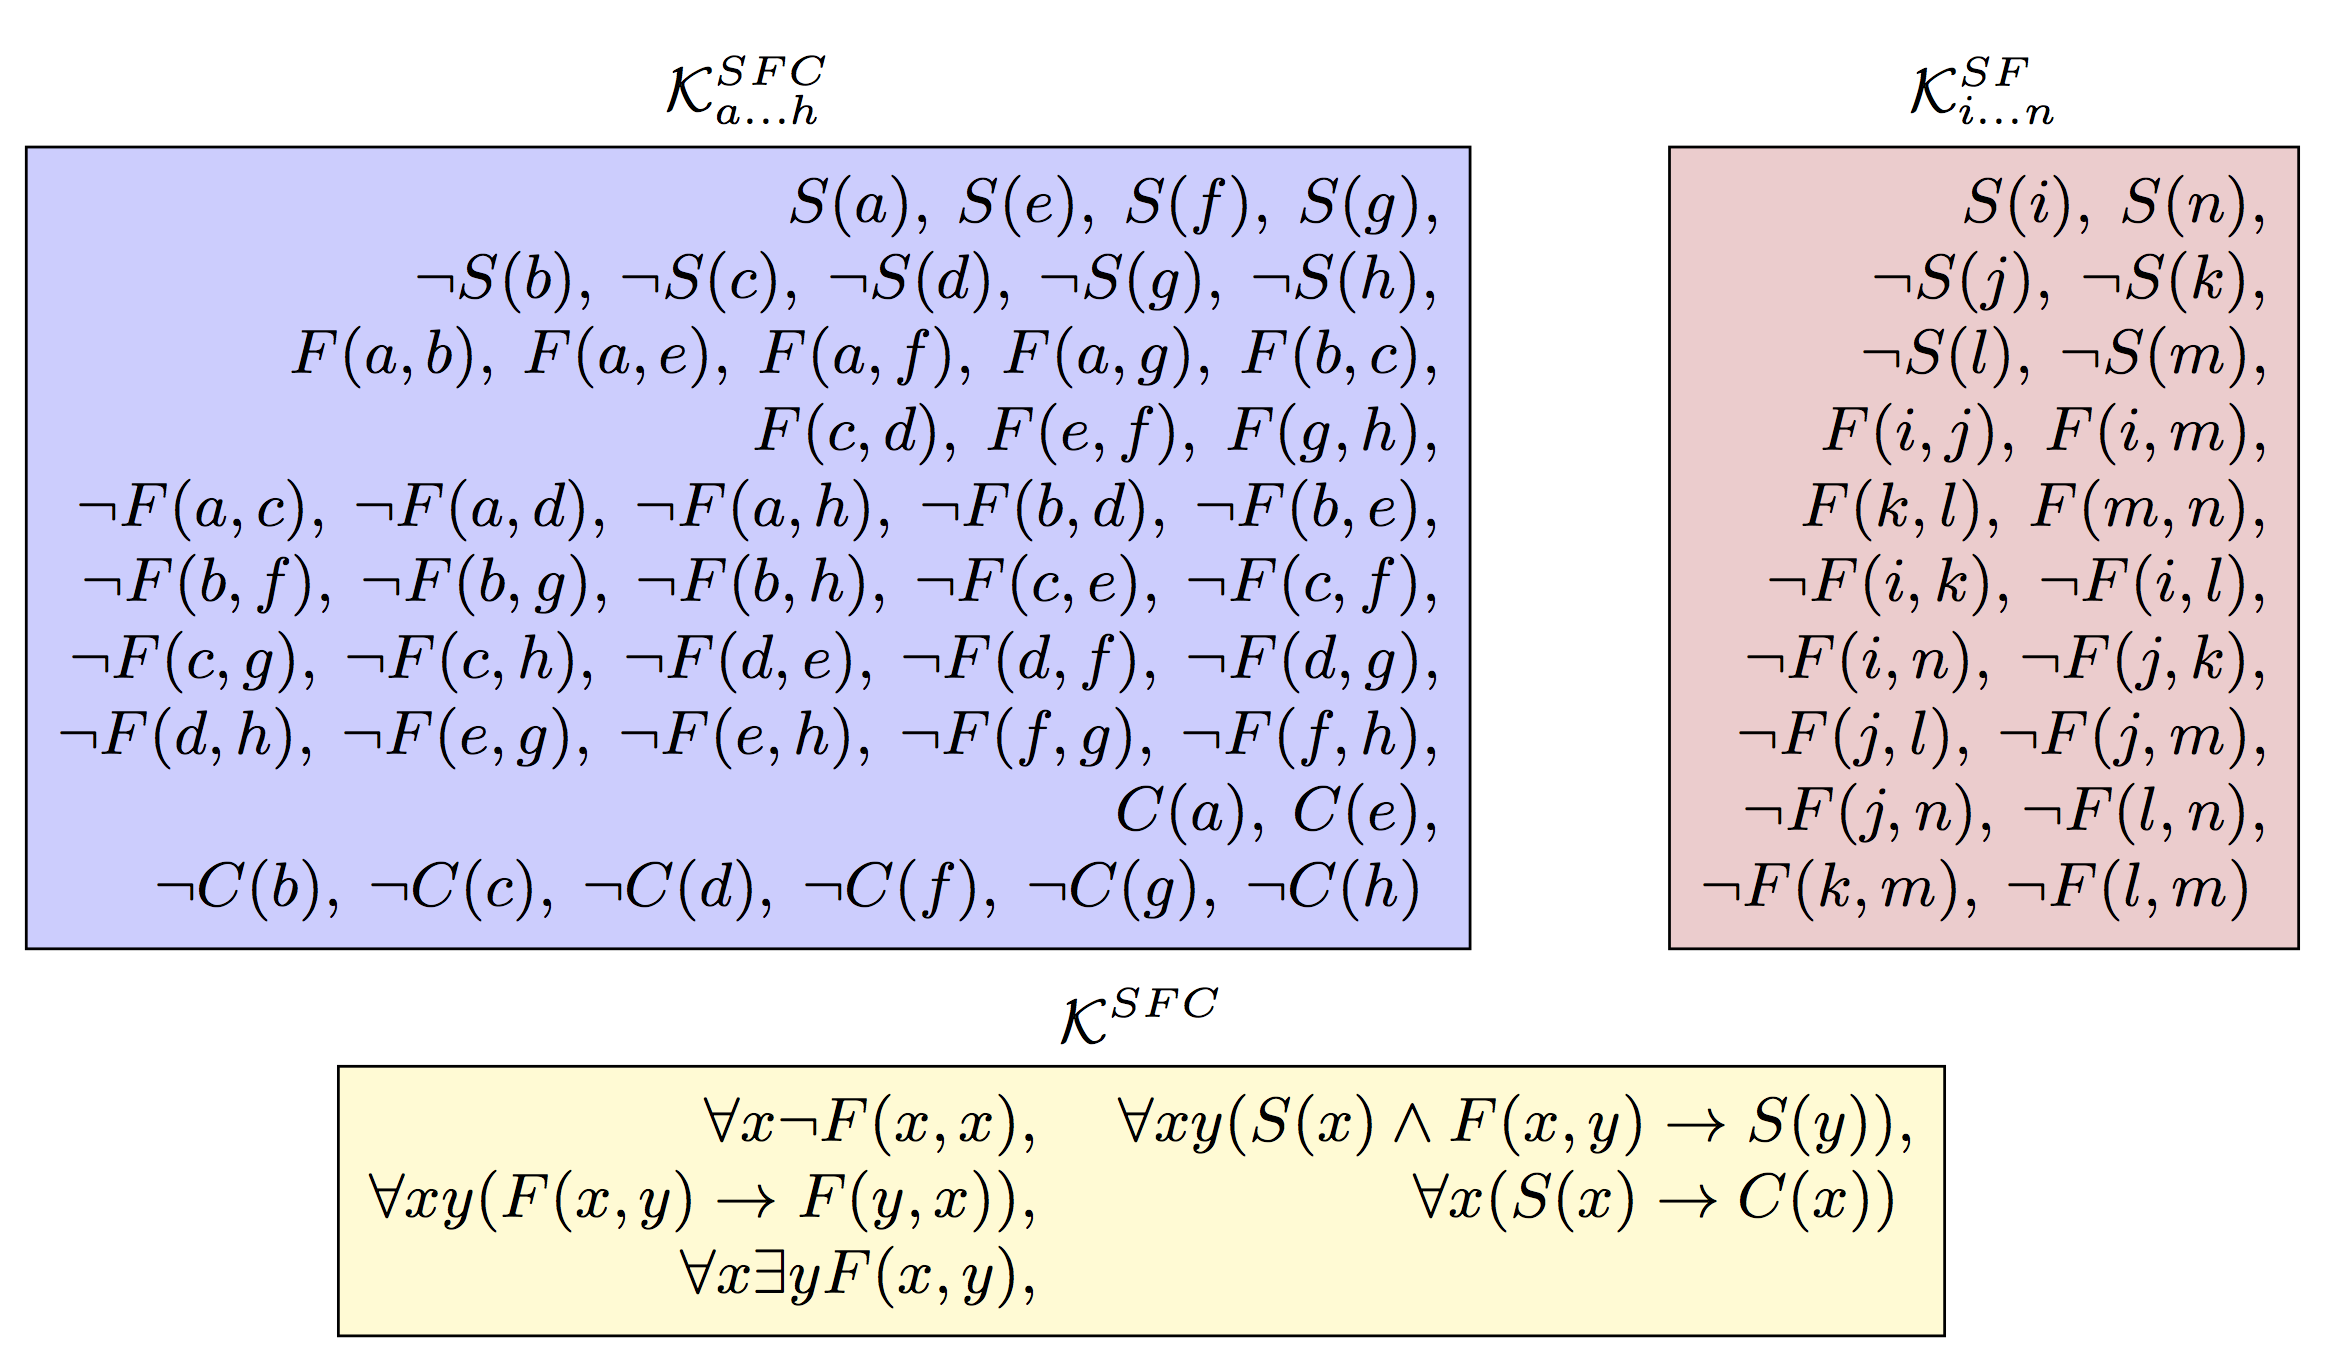
\includegraphics[width=.45\textwidth]{img/example.png}
    \caption{Friends and Smokers}
    \label{fig:example}
\end{figure}
